\phantomsection
\section*{6 线性映射基本定理}
\addcontentsline{toc}{section}{6 线性映射基本定理}

\vspace{2ex}

\centerline{\heiti A组}
\begin{enumerate}
    \item
\end{enumerate}

\centerline{\heiti B组}
\begin{enumerate}
    \item \begin{enumerate}
              \item 证明:$ \forall p_1(x), p_2(x) \in \mathbf{R}[x]_n,\enspace \forall k_1, k_2 \in \mathbf{R} $,有
                    \begin{align*}
                        \sigma(k_1 p_1 + k_2 p_2) & = (k_1 p_1(x) + k_2 p_2(x))'                                    \\
                                                  & = k_1 p_1'(x) + k_2 p_2'(x) = k_1 \sigma(p_1) + k_2 \sigma(p_2)
                    \end{align*}
                    因此 $ \sigma $ 是 $ \mathbf{R}[x]_n $ 上的线性变换.

              \item \begin{gather*}
                        \begin{aligned}
                            \im \sigma & = \spa(\sigma(1), \sigma(x), \sigma(x^2), \ldots, \sigma(x^{n - 1})) \\
                                       & = \spa(1, 2x, \ldots, (n - 1) x^{n - 2})                             \\
                                       & = \spa(1, x, \ldots, x^{n - 2})
                        \end{aligned} \\
                        r(\sigma) = n - 1
                    \end{gather*}
                    可知 $ \sigma $ 不是单射,因此不可逆.

              \item 由 $ \sigma(p(x)) = 0 $ 可知 $ p(x) = c $(常数). 因此 $ \ker \sigma = \spa(1),\enspace \dim \ker \sigma = 1 $.

              \item \begin{gather*}
                        r(\sigma) + \dim \ker \sigma = (n - 1) + 1 = n \\
                        \im \sigma + \ker \sigma = \spa(1, x, \ldots, x^{n - 2}) = \im \sigma \neq \mathbf{R}[x]_n
                    \end{gather*}
          \end{enumerate}

    \item \begin{enumerate}
              \item 可能. 例如 $ \sigma(x, y) = (x + y, x + y) $.
                    \begin{gather*}
                        \im \sigma = \spa(\vec{e}_1 + \vec{e}_2) \\
                        \ker \sigma = \spa(\vec{e}_1 - \vec{e}_2) \\
                        \im \sigma \cap \ker \sigma = \{\vec{0}\}
                    \end{gather*}

              \item 可能. 例如 $ \sigma(x, y, z) = (x - y, x - y, x - y) $.
                    \begin{gather*}
                        \im \sigma = \spa((1, 1, 1)) \\
                        \ker \sigma = \spa((1, 1, 1), (1, 1, 0)) \\
                        \im \sigma \subseteq \ker \sigma
                    \end{gather*}

              \item 可能. 例如 $ \sigma(x, y) = (x - y, x - y) $.
                    \begin{gather*}
                        \im \sigma = \ker \sigma = \spa((1, 1))
                    \end{gather*}

              \item 可能. 例如 $ \sigma(x, y) = (x, x - y) $.
                    \begin{gather*}
                        \im \sigma = \mathbf{R}^2 \\
                        \ker \sigma = \{\vec{0}\} \\
                        \ker \sigma \subseteq \im \sigma
                    \end{gather*}
          \end{enumerate}

    \item \begin{enumerate}
              \item 错误. 一个反例为 $ \sigma(x_1, x_2) = (x_1 - x_2, x_1 - x_2) $,则 $ \im \sigma + \ker \sigma = \spa((1, 1)) $.

              \item 正确. $ \im \sigma + \ker \sigma \subseteq V $,此时 $ \dim(\im \sigma + \ker \sigma) = \dim \im \sigma + \dim \ker \sigma - 0 = \dim V $,所以 $ \im \sigma + \ker \sigma = V $.

              \item \label{item:6:B:2:3}
                    错误. $ \forall \alpha \in V $ 有
                    \[ (\sigma_1 + \sigma_2)(\alpha) = \sigma_1(\alpha) + \sigma_2(\alpha) \in \sigma_1(V) + \sigma_2(V) \]
                    所以
                    \[ (\sigma_1 + \sigma_2)(V) \subseteq \sigma_1(V) + \sigma_2(V) \]
                    但上式中等号不一定成立. 反例:$ V = \mathbf{R}^3 $ 上的线性变换 $ \sigma_1, \sigma_2 $ 关于 $ \mathbf{R}^3 $ 的基 $ \vec{e}_1, \vec{e}_2, \vec{e}_3 $ 的像分别为
                    \begin{gather*}
                        \sigma_1(\vec{e}_1) = \vec{e}_1,\enspace \sigma_1(\vec{e}_2) = \sigma_1(\vec{e}_3) = \vec{e}_2 \\
                        \sigma_2(\vec{e}_1) = \vec{e}_1,\enspace \sigma_2(\vec{e}_2) = \sigma_2(\vec{e}_3) = \vec{e}_3 \\
                        \sigma_1(V) = \spa(\vec{e}_1, \vec{e}_2),\enspace \sigma_2(V) = \spa(\vec{e}_1, \vec{e}_3) \\
                        \sigma_1(V) + \sigma_2(V) = \spa(\vec{e}_1, \vec{e}_2, \vec{e}_3) = \mathbf{R}^3
                    \end{gather*}
                    而
                    \begin{gather*}
                        (\sigma_1 + \sigma_2)(\vec{e}_1) = \vec{e}_1 + \vec{e}_1 = 2 \vec{e}_1 \\
                        (\sigma_1 + \sigma_2)(\vec{e}_2) = (\sigma_1 + \sigma_2)(\vec{e}_3) = \vec{e}_2 + \vec{e}_3 \\
                        (\sigma_1 + \sigma_2)(V) = \spa(\vec{e}_1, \vec{e}_2 + \vec{e}_3) \neq \mathbf{R}^3
                    \end{gather*}

              \item 错误. $ (I - \sigma)(V) + \sigma(V) \subseteq V $,等号不一定成立,原因同 \ref*{item:6:B:2:3},此时只需将 $ I - \sigma $ 视作 $ \sigma_1 $,将 $ \sigma $ 视作 $ \sigma_2 $.
          \end{enumerate}

    \item 证明:\begin{enumerate}
              \item 由于 $ \ker \sigma = \im \sigma $,由 $ \dim \im \sigma + \dim \ker \sigma = \dim V $ 可得.

              \item 设 $ \beta_1, \ldots, \beta_n $ 为 $ V $ 的一组基,则
                    \[ \im \sigma = \spa(\sigma(\beta_1), \ldots, \sigma(\beta_n)) = \ker \sigma \]
                    设 $ \sigma(\beta_1), \ldots, \sigma(\beta_{\frac{n}{2}}) $ 为 $ \im \sigma $ 的基,则可以证明
                    \[ \sigma(\beta_1), \ldots, \sigma(\beta_{\frac{n}{2}}), \beta_1, \ldots, \beta_{\frac{n}{2}} \]
                    线性无关,且 $ \sigma $ 在此基下的矩阵即为所求的形式.
          \end{enumerate}

    \item \begin{enumerate}
              \item 在. 因为
                    \[ \sigma(\alpha_1) = -2 \sigma(\sigma_2) + \sigma(\alpha_3) = \sigma(-2 \alpha_2 + \alpha_3) \]
                    同构映射 $ \sigma $ 可逆. 所以
                    \[ \alpha_1 = -2 \alpha_2 + \alpha_3 \in \spa(\alpha_2, \alpha_3) \]
          \end{enumerate}

    \item 我们仅对 $ n = 3 $ 的情况给出证明. % TODO P117/7

          先证 $ \sigma $ 是线性映射. $ \forall p(x), q(x) \in \mathbf{R}[x]_3,\enspace \forall k_1, k_2 \in \mathbf{R} $ 有
          \begin{align*}
                  & \sigma(k_1 p(x) + k_2 q(x))                                                 \\
              ={} & (k_1 p(c_1) + k_2 q(c_1), k_1 p(c_2) + k_2 q(c_2), k_1 p(c_3) + k_2 q(c_3)) \\
              ={} & k_1(p(c_1), p(c_2), p(c_3)) + k_1(q(c_1), q(c_2), q(c_3))                   \\
              ={} & k_1 \sigma(p(x)) + k_2 \sigma(q(x))
          \end{align*}

          再证 $ \sigma $ 是双射,即 $ \forall (d_1, d_2, d_3) \in \mathbf{R}^3 $,存在唯一的
          \[ p(x) = a + bx + cx^2 \in \mathbf{R}[x]_3 \]
          使 $ \sigma(p(x)) = (d_1, d_2, d_3) $. 根据
          \[ \sigma(p(x)) = (p(c_1), p(c_2), p(c_3)) \]
          以及 $ \sigma(p(x)) = (d_1, d_2, d_3) $,有
          \[ \begin{cases}
                  a + bc_1 + cc_1^2 = d_1 \\
                  a + bc_2 + cc_2^2 = d_2 \\
                  a + bc_3 + cc_3^3 = d_3
              \end{cases} \]
          方程组是关于未知元 $ a, b, c $ 的三元线性非齐次方程组,其中 $ c_1, c_2, c_3 $ 是互异的实常数. 用高斯消元法,易将其增广矩阵变换为下列阶梯形矩阵,即
          \begin{align} % TODO 增广矩阵
                             & \begin{pmatrix}
                                   1 & c_1 & c_1^2 & \Bigm| & d_1 \\
                                   1 & c_2 & c_2^2 & \Bigm| & d_2 \\
                                   1 & c_3 & c_3^3 & \Bigm| & d_3
                               \end{pmatrix} \notag                                                             \\
              \implies \quad & \begin{pmatrix}
                                   1 & c_1 & c_1^2     & \Bigm| & d_1                                                         \\[1ex]
                                   0 & 1   & c_2 + c_1 & \Bigm| & \dfrac{d_1 - d_2}{c_1 - c_2}                                \\[2ex]
                                   0 & 0   & c_3 - c_2 & \Bigm| & \dfrac{d_3 - d_1}{c_3 - c_1} - \dfrac{d_2 - d_1}{c_2 - c_1}
                               \end{pmatrix} \label{item:6:B:6:1}
          \end{align}
          阶梯性矩阵 \ref*{item:6:B:6:1}(其中 $ c_3 - c_2, c_3 - c_1, c_2 - c_1 $ 均为非零常数)对应的方程组有唯一解 $ a, b, c $,即存在唯一的
          \[ p(x) = a + bx + cx^2 \in \mathbf{R}[x]_3 \]
          使得 $ \sigma(p(x)) = (d_1, d_2, d_3) $ 成立. 所以 $ \sigma $ 是线性双射,即 $ \mathbf{R}[x]_3 $ 到 $ \mathbf{R}^3 $ 的同构映射.
\end{enumerate}

\centerline{\heiti C组}
\begin{enumerate}
    \item 证明:必要性:$ \forall \alpha \in V $,由 $ \sigma $ 可逆,存在唯一的 $ \beta \in V $ 使得 $ \sigma(\beta) = \alpha $ 且 $ \beta = \beta_1 + \beta_2 $,其中 $ \beta_1 \in W_1 $,$ \beta_2 \in W_2 $. 于是
          \[ \alpha = \sigma(\beta) = \sigma(\beta_1) + \sigma(\beta_2) \in \sigma(W_1) + \sigma(W_2) \]
          所以 $ V \subseteq \sigma(W_1) + \sigma(W_2) $.

          $ \sigma(W_1), \sigma(W_2) $ 都是 $ V $ 的子空间,它们的和也是 $ V $ 的子空间. 所以 $ \sigma(W_1) + \sigma(W_2) \subseteq V $,故 $ V = \sigma(W_1) + \sigma(W_2) $.

          充分性:$ \forall \alpha \in V = \sigma(W_1) + \sigma(W_2) $,$ \exists \alpha_i \in \sigma(W_i) $ 且 $ \exists \beta_i \in W_i $ 使 $ \alpha_i = \sigma(\beta_i) $($ i = 1, 2 $)使得
          \[ \alpha = \alpha_1 + \alpha_2 = \sigma(\beta_1) + \sigma(\beta_2) = \sigma(\beta_1 + \beta_2) = \sigma(\beta) \]
          其中 $ \beta = \beta_1 + \beta_2 \in W_1 + W_2 = V $,所以 $ \sigma $ 为满射.

          由于 $ n $ 维线性空间上的线性映射为满射时也必为单射,从而必是双射,所以 $ \sigma $ 可逆.

    \item 证明:先证右边. 由于 $ \sigma(V_1) \subseteq V_2 $,所以 $ (\tau \sigma)(V_1) \subseteq \tau(V_2) $,如下图所示. 因此
          \[ \dim(\tau \sigma)(V_1) \leqslant \dim \tau(V_2) \]
          即 $ r(\tau \sigma) \leqslant r(\tau) $.
          \begin{figure}[H]
              \centering
              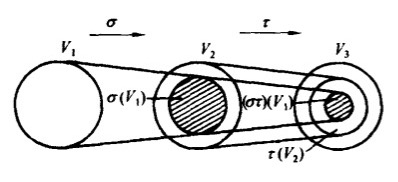
\includegraphics[scale=.5]{figs/6C.2.1.jpg}
          \end{figure}
          又因为 $ (\tau \sigma)(V_1) = \tau(\sigma(V_1)) $,所以又有
          \[ \dim(\tau \sigma)(V_1) \leqslant \dim \sigma(V_1) \]
          即 $ r(\tau \sigma) \leqslant r(\sigma) $.

          再证左边. 由线性映射维数公式,
          \begin{gather*}
              r(\tau) + \dim \ker \tau = n \\
              r(\tau \sigma) + \dim \ker(\tau \sigma) = m
          \end{gather*}
          又 $ \dim \ker(\tau \sigma) \leqslant \dim \ker \tau $,所以
          \[ m - r(\tau \sigma) = \dim \ker(\tau \sigma) \leqslant \dim \ker \tau \]
          代入线性映射维数公式,得 $ \dim \ker \tau = n - r(\tau) \geqslant m - r(\sigma) $,即
          \begin{align*}
              r(\tau \sigma) & \geqslant m + r(\tau) - n         \\
                             & \geqslant r(\sigma) + r(\tau) - n
          \end{align*}

    \item 证明:由于 $ \forall \beta \in (\sigma + \tau)(V_1),\enspace \exists \alpha \in V_1 $ 使 $ \beta = (\sigma + \tau)(\alpha) = \sigma(\alpha) + \tau(\alpha) \in \sigma(V_1) + \tau(V_1) $,所以
          \[ (\sigma + \tau)(V_1) \subseteq \sigma(V_1) + \tau(V_1) \]
          因此
          \begin{align*}
              \dim(\sigma + \tau)(V_1) & \leqslant \dim(\sigma(V_1) + \tau(V_1))     \\
                                       & \leqslant \dim \sigma(V_1) + \dim \tau(V_1)
          \end{align*}

    \item 证明:\begin{enumerate}
              \item \label{item:6:C:4:1}
                    $ \forall \sigma \in \mathcal{L}(V, V) $,则 $ I - \sigma \in \mathcal{L}(V, V) $. $ \forall \alpha \in (I - \sigma)(V),\enspace \exists \beta \in V $,有
                    \begin{gather*}
                        \alpha = (I - \sigma)(\beta) = \beta - \sigma(\beta) \\
                        \sigma(\alpha) = \sigma(\beta - \sigma(\beta)) = \sigma(\beta) - \sigma^2(\beta)
                    \end{gather*}
                    而由于 $ \sigma^2 = \sigma $,所以 $ \sigma(\alpha) = \vec{0} $,于是 $ \alpha \in \ker \sigma $,因此 $ (I - \sigma)(V) \subseteq \ker \sigma $.

              \item 利用 $ r(\sigma + \tau) \leqslant r(\sigma) + r(\tau) $ 和 $ r(\sigma) + \dim \ker \sigma = n $,由 \ref*{item:6:C:4:1} 可得
                    \begin{equation} \label{eq:6:C:4:2:1}
                        r(I - \sigma) + r(\sigma) \leqslant n
                    \end{equation}
                    又因为
                    \begin{equation} \label{eq:6:C:4:2:2}
                        r(I - \sigma) + r(\sigma) \geqslant r(I - \sigma + \sigma) = r(I) = n
                    \end{equation}
                    于是由\autoref{eq:6:C:4:2:1} 和\autoref{eq:6:C:4:2:2} 即可得到 $ r(I - \sigma) + r(\sigma) = n $.
          \end{enumerate}

    \item 证明:\begin{enumerate}
              \item \label{item:6:C:5:1}
                    $ \forall \alpha \in \im \sigma,\enspace \exists \beta \in V $ 使得 $ \sigma(\beta) = \alpha $. 由 $ \sigma^2 = \theta $ 可得 $ \sigma(\alpha) = \sigma^2(\beta) = \vec{0} $,因此 $ \alpha \in \ker \sigma $,从而 $ \im \sigma \subseteq \ker \sigma $. 于是我们得到
                    \[ n = \dim \im \sigma + \dim \ker \sigma \geqslant 2 \dim \im \sigma \]
                    即 $ \dim \im \sigma \leqslant \dfrac{n}{2} $.

              \item 由 \ref*{item:6:C:5:1} 可知,方程组 $ AX = \vec{0} $ 的基础解系含有 $ n - r(A) = \dim \ker \sigma \geqslant \dfrac{n}{2} $ 个解向量,所以结论成立.
          \end{enumerate}

    \item 假设 $ \alpha_1, \alpha_2, \ldots, \alpha_n \in \mathbf{F} $ 是 $ \mathbf{F} $ 作为数域 $ \mathbf{K} $ 上的线性空间的一组基,$ \beta_1, \ldots, \beta_m \in \mathbf{E} $ 是 $ \mathbf{E} $ 作为数域 $ \mathbf{F} $ 上的线性空间的一组基,则现在对于任意的 $ \beta \in \mathbf{E} $,都存在 $ k_1, \ldots, k_m \in \mathbf{F} $ 使得 $ \beta = \displaystyle\sum_{i = 1}^{m} k_i \beta_i $.

          而对于每一个 $ k_i \in \mathbf{F},\enspace i = 1, 2, \ldots, m $,存在 $ l_{ij} \in \mathbf{K},\enspace j = 1, 2, \ldots, n $ 使得 $ k_i = \displaystyle\sum_{j = 1}^{n} l_{ij} a_j $. 于是
          \[ \beta = \sum_{i = 1}^{m} \sum_{j = 1}^{n} l_{ij} \alpha_j \beta_i \]
          这说明对任意的 $ \beta \in \mathbf{E} $,都可由
          \[ \alpha_1 \beta_1, \ldots, \alpha_1 \beta_m, \alpha_2 \beta_1, \ldots, \alpha_n \beta_m \]
          这 $ mn $ 个向量线性表出,其中线性表出的系数都属于最小的数域 $ \mathbf{K} $.

          同时,如果假设 $ l_{ij} \in \mathbf{K} $ 满足 $ \displaystyle\sum_{i = 1}^{m} \displaystyle\sum_{j = 1}^{n} l_{ij} \alpha_j \beta_i = 0 $,则
          \[ \sum_{i = 1}^{m} \left(\sum_{j = 1}^{n} l_{ij} \alpha_j\right) \beta_i = 0 \]
          利用 $ \beta_1, \ldots, \beta_m $ 的线性无关性可得 $ \displaystyle\sum_{j = 1}^{n} l_{ij} \alpha_j = 0 $,再结合 $ \alpha_1, \ldots, \alpha_n $ 线性无关可得 $ l_{ij} = 0 $,这就说明 $ \alpha_1 \beta_1, \ldots, \alpha_1 \beta_m, \alpha_2 \beta_1, \ldots, \alpha_n \beta_m $ 在数域 $ \mathbf{K} $ 是线性无关的.

          综上,$ \alpha_1 \beta_1, \ldots, \alpha_1 \beta_m, \alpha_2 \beta_1, \ldots, \alpha_n \beta_m $ 就是 $ \mathbf{E} $ 作为 $ \mathbf{K} $ 的线性空间的一组基,从而这个线性空间是 $ mn $ 维的.
\end{enumerate}

\clearpage
